
\section{Sentiment Representation Structures}

\subsection{Ekman's Six Basic Emotions}

There is no universally accepted model for representing sentiments, but a standard for classifying emotions in a categorical model is using Ekmans six basic emotions \cite{Ekman}. These are identified as Anger, Disgust, Fear, Happiness, Sadness and Surprise. Since there are only six discrete classes in which emotions can be placed, this can be argued to be very subjective when classifying \cite{emoBank}, but are very useful in portraying a general result back to user rather than numeric values. Other ways of representing emotion in discrete classes exist, such as Izards 12 categories, but they are not as popular as Ekman's representation and have less literature available \cite{izard1993stability} .

\subsection{Valence}
A very common way to classify phrases and sentences in sentiment analysis is to analyse the Valence of the text, as already briefly discussed \cite{frijda1986emotions}.

The Valence of a piece of text is how positive or negative is perceived to be, usually rated on a scale between 0 and 1, with 0 being negative.
Using Valence in a machine learning context is very useful, since many textual datasets exist that are already split into how positive a piece of text is, such as product or movie reviews which are frequently accompanied by a star rating. There is plenty of previous projects that use this as a way to represent emotion, taking in input text and outputting a Valence value usually on a numeric scale, so this is a good base to structure a more complex model on.

\subsection{Valence Arousal Dominance Structure}

The Valence-Arousal-Dominance (VAD) structure provides a 3D representation for emotions, with each variable being defined as follows \cite{VAD}:
\begin{itemize}
    \item Valence- How positive or negative the statement is (as before).
    \item Arousal- Degree of calmness or excitement, the energy of the statement. 
    \item Dominance- Degree of control over a situation.
\end{itemize}

This structure provides the extra information about an emotion that is needed for a more in depth analysis of text, so will be used as the scale to analyse input text with for this project.

Using VAD values allows for easy representation into the Ekman six basic emotions as well, using a standard for translating between them as shown in Table \ref{ekmansTable}.


\begin{table}[ht]
\caption{Ekmans emotions mapped to VAD values \cite{VADMapping}, with values ranging from 0 to 5}
\centering
\begin{tabular}{ |c|c|c|c|c|c|c| } 
 \hline
  & Anger & Disgust & Fear & Happiness & Sadness & Surprise \\ 
 \hline                        
 Valence & 1.23 & 1 & 0.9 & 4.53 & 0.93 & 3.5\\ 
 Arousal & 3.98 & 3.38 & 4 & 3.78 & 1.83 & 4.18\\ 
 Dominance & 3.13 & 2.78 & 1.43 & 3.65 & 1.68 & 2.18\\ 
 \hline
\end{tabular}
\label{ekmansTable}
\end{table}
\pagebreak
\section{Datasets}

There are two suitable datasets for this task which rank text using a VAD structure.

\subsection{Bag-of-Words}

The bag-of-words dataset contains 14,000 English words, each with a specific VAD value assigned \cite{wordsData}. Building a prediction model with this dataset would lose any context in which the words are in within a sentence as they would be treated each as separate entities, so is not ideal for a prediction task, but using it to create a lexicon-based bag of words style model will be investigated.

\begin{figure}[h]
\centering
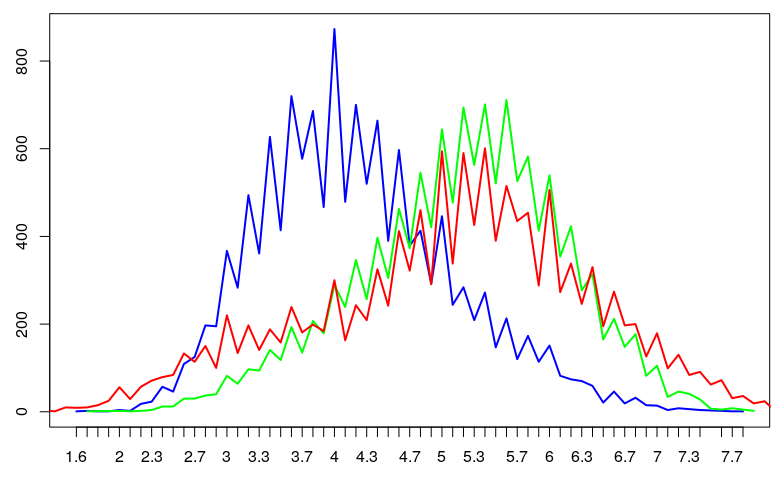
\includegraphics[scale=0.4]{graphs/lexiconDist.png}
\caption{Frequency of words over each dimension in bag-of-words dataset R: Valence, B: Arousal, G: Dominance. The dataset ranks the words on a scale between 0 and 10, which is adjusted for use with the EmoBank dataset}
\label{lexiconGraph}
\end{figure}

As we can see from Figure \ref{lexiconGraph} there is a bias in the data for each dimension, and the average value for the Arousal dimension is noticeably lower than the other two. Whether this affects the suitability of this dataset for use in building a prediction model will be explored further.

\subsection{EmoBank}
This dataset is the most important one for this project, as it contains 10,000 English sentences covering multiple genres, all annotated with their own VAD values \cite{emoBank}.

This dataset contains values for each sample sentence from both the writer and the reader of the text, but due to the findings in the paper accompanying it \cite{emoBank}, only the values given by the reader will be used, as it concluded that this perspective has higher emotionality and therefore they should be easier to build a more accurate model with.

Many existing sentiment analysis tools train over very large datasets, scraping information from things such as movie reviews \cite{socher2013recursive} or from Tweets \cite{towardsDS}, and so usually have above 100,000 samples to train from. In this case, the EmoBank dataset only contains 10,000 sentences, and whether this is a setback will have to be taken into account. These larger datasets could not be used in this case since they are not annotated in a way that allows a more complex emotion to be calculated, since they are usually only scored by their Valence values. 

We can see from Figure \ref{dist:vad} that most of the EmoBank data lies in the middle of the dataset, meaning that there is an imbalance in data. This can cause issues for building a prediction model from, as many prediction models will overfit on the majority class or range of values, predicting the most likely values every time. Dealing with this to be able to use the Emobank dataset in the most effective way will also be explored further.

\begin{figure}[h]
\centering
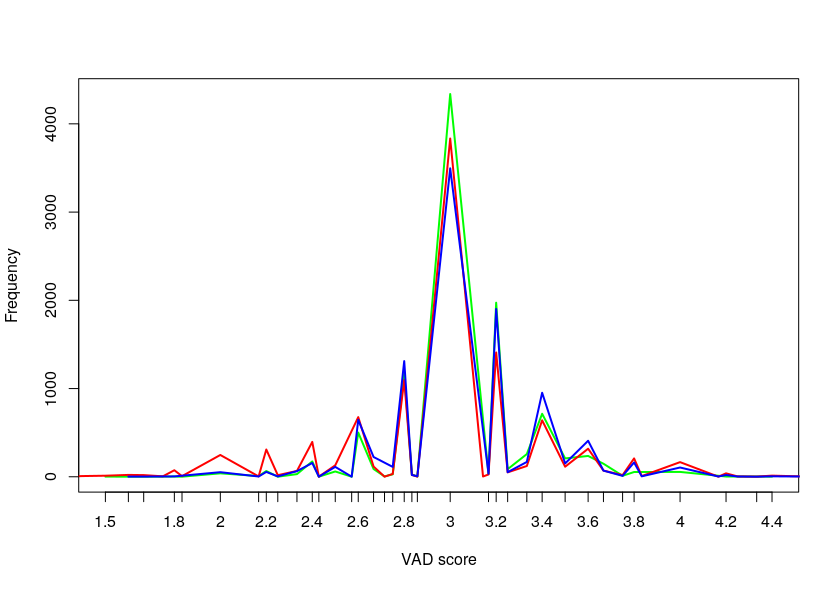
\includegraphics[scale=0.5]{graphs/VADdistribution.png}
\caption{Graph showing data distribution over the Emobank Dataset. R: Valence, B: Arousal, G: Dominance}
\label{dist:vad}
\end{figure}
